\section{Evolúciós játékok}

\iffalse 
Általános bemutatás.
Összehasonlítás a "klasszikus" játékelmélettel - külön alcím/fejezet?
 racionális játékosok <-> nem racionális játékosok
 dinamikus - mit jelent?
\fi
\subsection{Klasszikus játékelméleti fogalmak}
A játékelmélet a matematika egyik interdiszciplináris ága, amely a különböző döntési vagy verseny helyzetekben résztvevő felek viselkedését tanulmányozza. Ezekben a \textit{játékokban} - többszereplős konfliktusos szituációkban - a választott stratégiák szorosan összefüggenek, mivel minden résztvevő döntése befolyásolja a többiek választásának eredményét is.\cite{wiki:gametheory} A \textit{játékosok} alapvető célja a nyereségük maximalizálása. A játékosok és a jutalom mibenléte tudományterületenként változó. A játékelmélet alkalmazható úgy a matematikában, közgazdaságtanban, mint a  szociológiában, biológiában felmerülő döntési problémák megoldására, modellezésére.

A játékokat különböző szempontok alapján több csoportra oszthatjuk. A játék lehet \textit{kooperatív}, ahol a játékosok külső hatásra koalíciókat alkotnak, vagy \textit{nem kooperatív}, ahol a résztvevők versenytársai egymásnak és ha létre is jön együttműködés, az önkéntes. 

\textit{Szimmetrikus} játékok esetén a haszon csak a választott stratégiától függ, a játékos személyétől nem. Ha a játékosok nem cserélhetőek fel anélkül, hogy a stratégiák nyereségén változtatnánk, \textit{aszimmetrikus} játékról beszélünk. A legismertebb kétszemélyes játékok, mint a későbbiekben tárgyalt fogolydilemma vagy héja-galamb játék, szimmetrikusak.

\subsubsection{Statikus és dinamikus játékok}
Az idő szerepe fontos osztályozási kritérium, eszerint beszélhetünk \textit{statikus} és \textit{dinamikus} játékokról. Statikus játékok legfontosabb tulajdonsága, hogy a játékosok már a játék elején, egymástól függetlenül döntenek. Dinamikus játékok esetén számít a lépések sorrendje, mivel a játékosok ismerik a többiek eddigi lépéseit. A utóbbi csoportba sorolják az ismételt játékokat is, amikor egy statikus játékot véges vagy végtelenszer megismételnek. Itt a résztvevők minden kör után megfigyelhetik a többiek eddigi lépéseit és az alapján választhatják meg a következő körben alkalmazott stratégiát. A két típust különbözőképpen ábrázoljuk. A nem-kooperatív statikus játékokat általában egy mátrix segítségével írjuk le, amelyről leolvasható az összes lehetséges kombináció eredménye. Ezt nevezzük \textit{normál alaknak}. Dinamikus játék esetén, az ún. \textit{extenzív alakban}, az egymás utáni lépéseket egy véges irányított fa ábrázolja, amely gyökere a kezdőállapot, ahonnan a fa minden pontjához pontosan egy úton lehet eljutni.

\subsubsection{Nash-egyensúly}
A játékelmélet egyik központi fogalma a Nash-egyensúly. Egy stratégia-együttes Nash-egyensúlyban van ha a csoportban egyik félnek sem érdemes eltérni az alkalmazott stratégiától, amennyiben egyik fél sem változtat a sajátján. Tekintsük \(G = ((N,S_i,u_i), i = 1,...,n)\) rendszert egy véges stratégia játék reprezentációjának, ahol \textit{N} a játékosok halmaza, \textit{n} pedig a játékosok száma. Minden \(i \in N\) játékos a \(S_i\) lépés-halmazból választhat. \(S = S_1 \times S_2 \times ... \times S_n\)  a játék összes kimenetelének halmaza, ahol \(s \in S\) egy stratégia-együttes. Minden \(i \in N\) játékos nyereségét a \(u_i:S \to \mathbb{R}\) hasznosságfüggvény írja le. Jelöljük \((s_i^*,s_i) = (s^*_1,...,s_i,...,s_n^*)\) -vel azt a stratégia-együttest, amelyet az \(s^*\)-ból kapunk ha az \textit{i} játékos stratégiáját kicseréljük \(s_i\)-re. Egy \(s^*\) stratégia-együttes Nash-egyensúlyban van, ha az \(u_i(s_i^*,s_i)\leq u_i(s^*) \) egyenlőtlenség igaz \(\forall i = 1,...,n, \forall s_i \in S_i, s_i \ne s_i^*\) esetén \cite{nash1951non}.

\subsection{Játékelmélet a biológiában}
A játékelmélet alkalmazása a biológiában az \textit{evolúciós játékelmélet}. Maynard Smith, a terület első és legismertebb alakja, kijelenti, hogy az addigi nézetekkel ellentétben, a játékosoknak nem kell kötelező módon racionálisan dönteniük, elegendő ha van egy stratégiájuk. A stratégia genetikailag örökölt jelleg, ami az egyed viselkedését befolyásolja. Sikerét az mutatja, hogy mennyire tud fennmaradni és milyen gyakorisággal jelenik meg más stratégiák között. A résztvevők szelekciós sikerét a \textit{fitnesz} fejezi ki (a szaporodásra való relatív esély). Az evolúciós játékok segítségével modellezhetjük a fajon belüli rivalizálást, a ragadozó-préda kapcsolatot de akár a gének vagy baktériumok közötti kölcsönhatásokat is. A klasszikus játékelmélettel ellentétben itt a stratégiák változásának dinamikájára helyeződik a hangsúly. Egészen egyszerű játékok esetén is megtörténik, hogy a hosszútávú eredmény nem a Nash-egyensúly, hanem rendszeres vagy rendszertelen oszcillálás \cite{nowak2004evolutionary}. Evolúciós játékokban az egyensúlyt az \textit{evolúciósan stabil stratégia} jelenti. Egy stratégia evolúciósan stabil, ha az azt alkalmazó populáció egy adott környezetben nem győzhető le semmilyen más alternatív, kezdetben kevés létszámú stratégiával.
 
Egyik legegyszerűbb játékelméleti modell két stratégiával és négy lehetséges eredménnyel dolgozik. A játékosok együttműködhetnek vagy defektálhatnak. Ha mindkét játékos kooperál nagyobb a nyereségük mintha mindketten defektálnának, de ha az egyik kooperál akkor a másiknak jobban megéri kihasználni azt és nem együttműködni. A kooperáló játékossal két dolog történhet: vagy az éri meg jobban ha ő is változtat a stratégián és nem hagyja, hogy kizsákmányolják, mint a jól ismert fogolydilemmában (ábra \ref{fig:prisoners}.), vagy még mindig akkor dönt jobban ha továbbra is együttműködik, ahogyan a héja-galamb játékban (ábra \ref{fig:hawkdove}.) történik. A kihívást a nyereségfüggvény helyes beállítása jelenti, hiszen attól függ, hogy egyik vagy másik játékhoz hasonlítjuk a természetben előforduló jelenségeket \cite{nowak2004evolutionary}.
 
\begin{minipage}{\linewidth}
	\centering
	\begin{multicols}{2}
		\begin{Figure}
			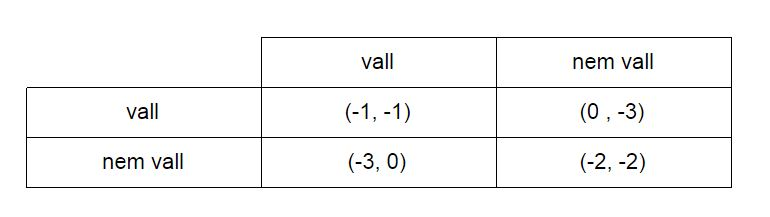
\includegraphics[width=\linewidth]{images/prisoners}
			\captionof{figure}{Fogolydilemma: két elkülönített fogoly dönthet, hogy hallgat vagy vall a másik ellen. A mátrix a nyereségeket (börtönben töltött évek) szemlélteti\label{fig:prisoners}}
		\end{Figure}
		\begin{Figure}
			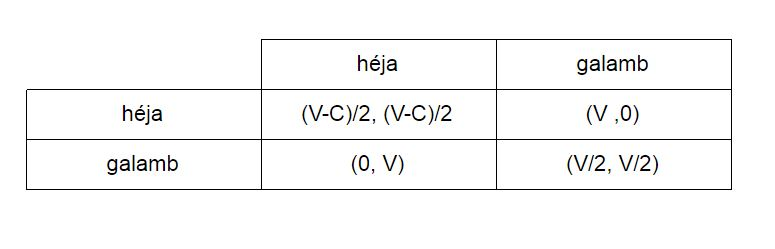
\includegraphics[width=\linewidth]{images/hawkdove}
			\captionof{figure}{Héja-galamb játék: két héja mindig megküzd a \textit{V} erőforrásért, de ennek költsége \textit{C}, két galamb osztozkodik, egy galamb pedig mindig átengedi az erőforrást a héjának. \label{fig:hawkdove}}
		\end{Figure}
	\end{multicols}
\end{minipage}

\subsubsection{Replikátor dinamika}
A replikátor dinamika az egyik módja a gyakoriság-függő szelekció vizsgálatának. A megközelítés egy heterogén populációt feltételez, véges számú stratégiával, ahol a növekedés arányos a fitnesszel. A játék dinamikája a 
\begin{equation}
\frac{dx_i}{dt} = x_i(f_i(x) - F(x))
\end{equation}
differenciálegyenlettel írható le, ahol \(x_i\) az \textit{i} stratégia gyakorisága, \(f_i(x)\) a stratégia várható nyeresége az \(x = (x_1,...,x_n)\) eloszlású populációban, \(F(x)\) pedig a populáció átlagos nyeresége.
Ez a dinamika átalakul ha térbeli játékokkal foglalkozunk, ahol a játékosok legtöbbször egy rácson helyezkednek el egy síkban és csak a szomszédokkal lépnek kapcsolatba. Számít emellett az is, hogy szinkron vagy aszinkron módon számoljuk ki a nyereségeket \cite{hummert2014evolutionary}. 

\subsubsection{Adaptív dinamika}
A replikátor dinamikával ellentétben, ahol nem esik szó mutációról, az adaptív dinamika egy mutáns egyed vagy egyedek fitneszét vizsgálja egy rezidens populációban. Mint már említettük, egy populáció akkor stabil ha egyetlen mutáns csoport stratégiája sem múlja felül a jelenleg alkalmazottat, feltéve ha az új egyedek aránya elég kicsi. Tehát a végeredmény függ a mutáns egyedek  kezdeti arányától. A dinamika a 
\begin{equation}
\frac{dx_i}{dt} = \frac{\partial}{\partial y_i}A(y,x), i = 1,...,n
\end{equation}
differenciálegyenlettel számítható ki \(y = x\)-ben, ahol \textit{x} az eredeti stratégia, \(y = x + h\) a mutáns stratégiája (\textit{x}-hez közel álló), \textit{A(y,x)} egy \textit{y} stratégiát \textit{x}-szel szemben játszó egyed nyeresége. A relatív nyereség az \(A(y,x) - A(x,x)\) \cite{hummert2014evolutionary}.
